%************************************************
\chapter{Reinforcement Learning for tuning of  Distillation Control Systems}\label{ch:rl_tuning} 
%************************************************
Despite a long history of research and innovation, tuning of feedback controllers in chemical plants remains a time-intensive and costly task. This pain point was made clear by our collaborators at BASF who regularly need to tune controllers for laboratory distillation columns. Their operators often spend weeks attempting to find the best tuning parameters for a new distillation column setup, which is unacceptable given the short timelines of process development.

In this chapter, the aim is to develop a workflow for tuning control systems of distillation columns. I begin by reviewing the literature in this domain before outlining a failed approach we took using reinforcement learning.  In the following chapter, I then transition to discuss our new approach, which relies on more rigorous dynamic simulation and Bayesian optimisation.

\section{Background}


\subsection{Distillation control basics}
A continuous distillation column separates a mixture of fluids by differences in their boiling points. As shown in Figure \ref{lv_config}, a mixture is fed to the input of a column at rate $F$ with composition $z_F$.  When the feed enters the column, it is heated by vapor flowing up from the reboiler. Inside the column are trays or packing designed to increase the surface area for contact between the liquid and the vapor. This causes the lower boiling component(s) to migrate to the top of the column as vapor, while the higher boiling component(s) migrate to the bottom. The purified vapor is condensed at the top of the column, and a portion is returned to the column as reflux $L$; the rest of the condensed vapor is collected as distillate $D$. Similarly, some of the bottom liquid is boiled up to vapor $V$, and the remainder is collected as bottoms $B$.

\begin{figure}[t]
  \centering
  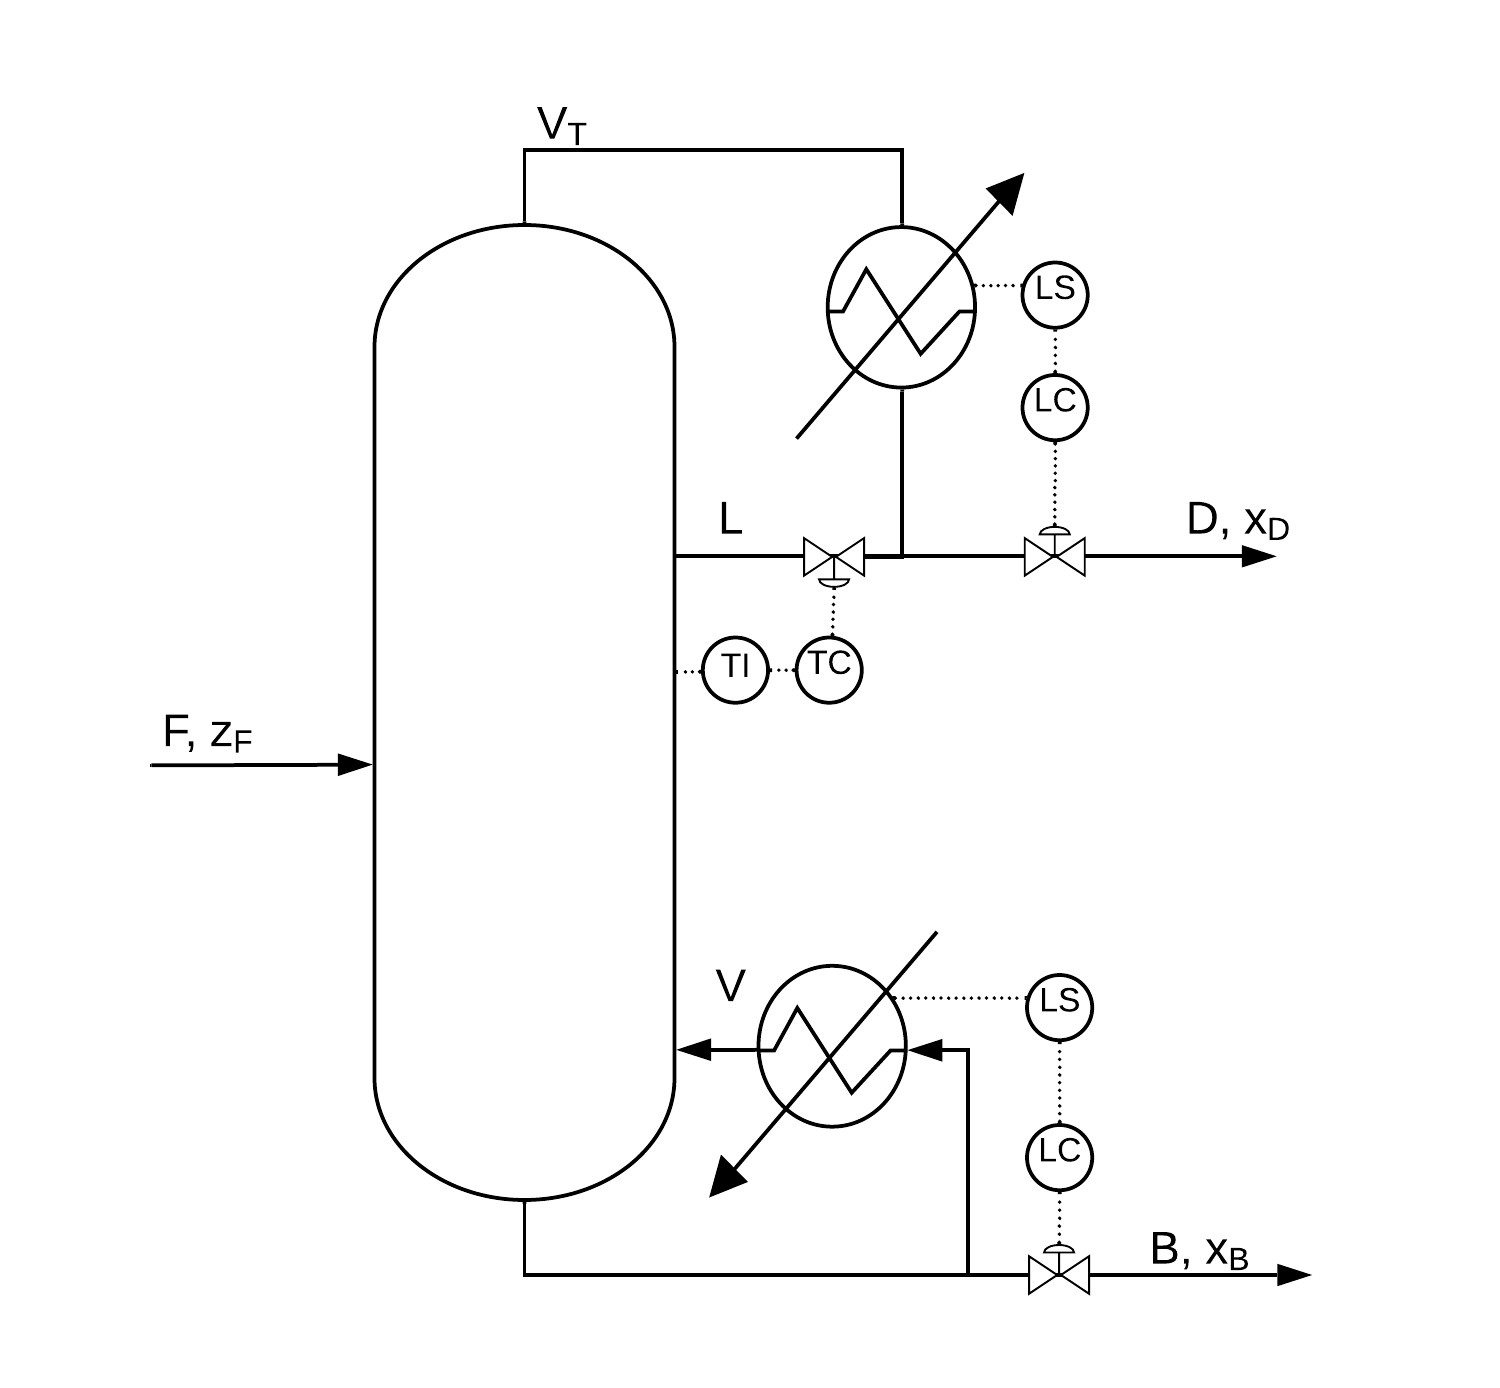
\includegraphics[height=0.3\textheight]{gfx/Chapter05/lv_configuration_inferential.png}
  \caption{Schematic of a distillation column with feed $F$, bottoms $B$, boilup $V$, reflux $L$ and distillate $D$.The  LV control configuration is used with an inferential composition controller. The level in the condenser and reboiler are controllers with the distillate and bottoms flows, respectively. Composition control can then be achieves with reflux or boilup, and in this case, reflux is used.}
  \label{lv_config}
\end{figure}

Distillation control schemes are designed to reject three common disturbances: changes in reboiler heating duty;  changes in condenser cooling duty; and changes in feed composition, rate or enthalpy \cite{Riggs2006}. All of these disturbances will affect the composition of the distillate and bottoms.  For example, a decrease in reboiler heating duty will reduce the vapor flow rate up the column.  As a result, the distillate composition will become less pure.\footnotemark   In the worst case, weeping can occur, where liquid flow prevents gas flow upwards and causes a drop in the purity of the distillate and bottoms streams. \footnotetext{This assumes that the distillate to feed ratio is kept constant, so the reflux decreases causing the distillate to become less pure.}

Feedback controllers are usually used to respond to these disturbances and maintain optimal operation of the column.  In the most general sense, a feedback controller receives a desired value of a control variable (CV) and keeps that variable constant through measurements and actuation. For example, a temperature controller on a hot water tank might use thermocouple measurements inside the tank to guide how it actuates a hot water inlet valve. Distillation columns have several potential control variables and potential actuators. This makes distillation a multiple input multiple output (MIMO) control problem. 

Approaches for designing MIMO control schemes can be broadly divided into those that use several decentralized single-input single-output (SISO) proportional integral derivative (PID) controllers\cite{Behroozsarand2012, Shen1994, Lin2006, Luyben1986} and those that design a single integrated controller \cite{Martin2013, Mesbah2017,Spielberg2019,Terzi2020}. In the decentralized approach, one controller might maintain the temperature of a particular tray in the distillation column by manipulating reflux rate while another holds the level in the reflux drum constant by changing distillate rate (see Figure \ref{lv_config}). It would be common to also have another controller on the reboiler or sump level \cite{Skogestad2007}. In contrast, the single integrated controller approach lumps all inputs and outputs into one central mathematical formulation, which can theoretically enable better rejection of disturbances \cite{Mesbah2017}. The most popular integrated controller formulation is model predictive control (MPC). MPC uses an internal model of the process to predict a series of discrete control actions that will lead to reaching the setpoints of all CVs.  However, in practice, many laboratory distillation columns still use decentralized control due to its simplicity.

% Instead of being used separately, MPC and decentralized PID control are often used in tandem. The PID controllers respond quickly to high frequency disturbances, while the MPC provides setpoints for the PID controllers that optimize the overall performance of the system \cite{Skogestad2007}. The MPC controller is often referred to as the supervisory control layer, while the PID controllers are called the regulatory control layer. Before a supervisory controller can be designed, the regulatory control layer needs to be properly designed. This starts with choosing controller pairings.

% In the literature, a specific combination of control pairings is called a configuration. Configurations are named based on the manipulated variables for composition control. For example, the LV configuration uses the reflux (L) and/or vapor boilup (V) streams as manipulated variables for composition control \cite{Skogestad2007}.  The remaining two degrees of freedom are used for level control; in the LV configuration, the condenser and reboiler levels are controlled by the distillate (D) and bottoms (B) flow rates, respectively. These level controllers respond to a wide variety of disturbances including fluctuations in the cooling duty of the condenser, changes in column pressure drop or changes in the heating duty of the reboiler.


% Each configuration has its own benefits and drawbacks based on the desired operating mode of the column (e.g., high vs. low reflux) and the type of disturbances observed. For example, the LV configuration is not preferred for high reflux ratios because the distillate flow will be very small, so it will have little influence on the condenser level \cite{Skogestad2007}. Furthermore, L and V are highly coupled, which degrades control performance \cite{Riggs2006}. Four common  control  configurations are shown in Table \ref{table:distillation_configurations}.

% \subsection{Choosing controller pairings} 
% \begin{table*}[t]
% 	\centering
% 	\caption{Comparison of control configurations for distillation columns. The following abbreviations are used for flows: L is reflux, V is vapor boilup, D is distillate and B is bottoms. S.S. means steady state.}
% 	\label{table:distillation_configurations}
% 		\begin{tabular}{ c c c }
% 			Configuration & Inputs for Level Control & Notes\\
% 			\hline
% 			L,V & D,B & Not good for high reflux ratios\cite{Skogestad2007}   \\
% 			D,B & L,V & Works at low relative volatility\cite{Finco1989} \\
% 			D,V & L,B & Large S.S. coupling, practically effective\cite{Riggs2006} \\
% 			L,B & D,V & Works well for high purity columns\cite{Skogestad2007} \\
% 		\end{tabular}
% \end{table*}
%  The challenge is that the combinatorial space for control configurations is large \cite{Shinskey1984}. If temperature control is used to control composition, sensors could theoretically be placed on any stage in a distillation column. If two level controllers and one temperature controller are used, there are $36N$ potential pairings, where $N$ is the number of stages.\footnotemark It is common for pilot plant columns to have 30 or more stages, so there are usually over 1000 potential pairings making brute force testing of all pairings infeasible.
%  \footnotetext{This is calculated by considering that there are four potential flow pairings (LV, DB, DV, LB) and five potential ratio pairings (double ratio, L/D-B, L/D-V, L/D-B, L-V/B, D-V/B) giving nine pairings. With single point temperature control, there are $4N$ pairings (two potential flows and two potential flows in ratio with feed paired with $N$ potential stages). This gives in total potential $9*4*N=36N$ pairings.}

% Therefore, engineers have attempted to predict the best pairings based on small amounts of data. Traditionally, the relative gain array (RGA) has been suggested to choose control pairings \cite{Shinskey1984,DeWal2001,Skogestad2007}. For a two-input two-output MIMO system, the RGA is defined by Equation \ref{eq:RGA} and \ref{eq:lambda}.

% \begin{equation} \label{eq:RGA}
% 	RGA = \begin{pmatrix} \lambda_{11} & \lambda_{12} \\ \lambda_{21} & \lambda_{22} \end{pmatrix}
% \end{equation}
% \begin{equation} \label{eq:lambda}
% 	\lambda_{11} = \frac{(\Delta y_1/\Delta u_1)_{u_2}}{(\Delta y_1/\Delta u_1)_{y_2}}
% \end{equation}

% The diagonal of the RGA represents the pairings. An input $u_1$ is paired with an output $y_1$, and another input $u_2$ is paired with output $y_2$. The parameter $\lambda_{11}$ is the ratio of the process gain without control to the process gain with control \cite{Riggs2006}. That is, the numerator represents how much $y_1$ changes when input 1 changes ($\Delta u_1$) while keeping input 2 constant (i.e., the second loop is left open).  The denominator represents how much $y_1$ changes when input 1 changes and the second loop is closed. Note that all other $\lambda$ values can be determined once $\lambda_{11}$ is specified for a 2x2 system \cite{Riggs2006}.

% %\begin{figure*}[bt]
% %  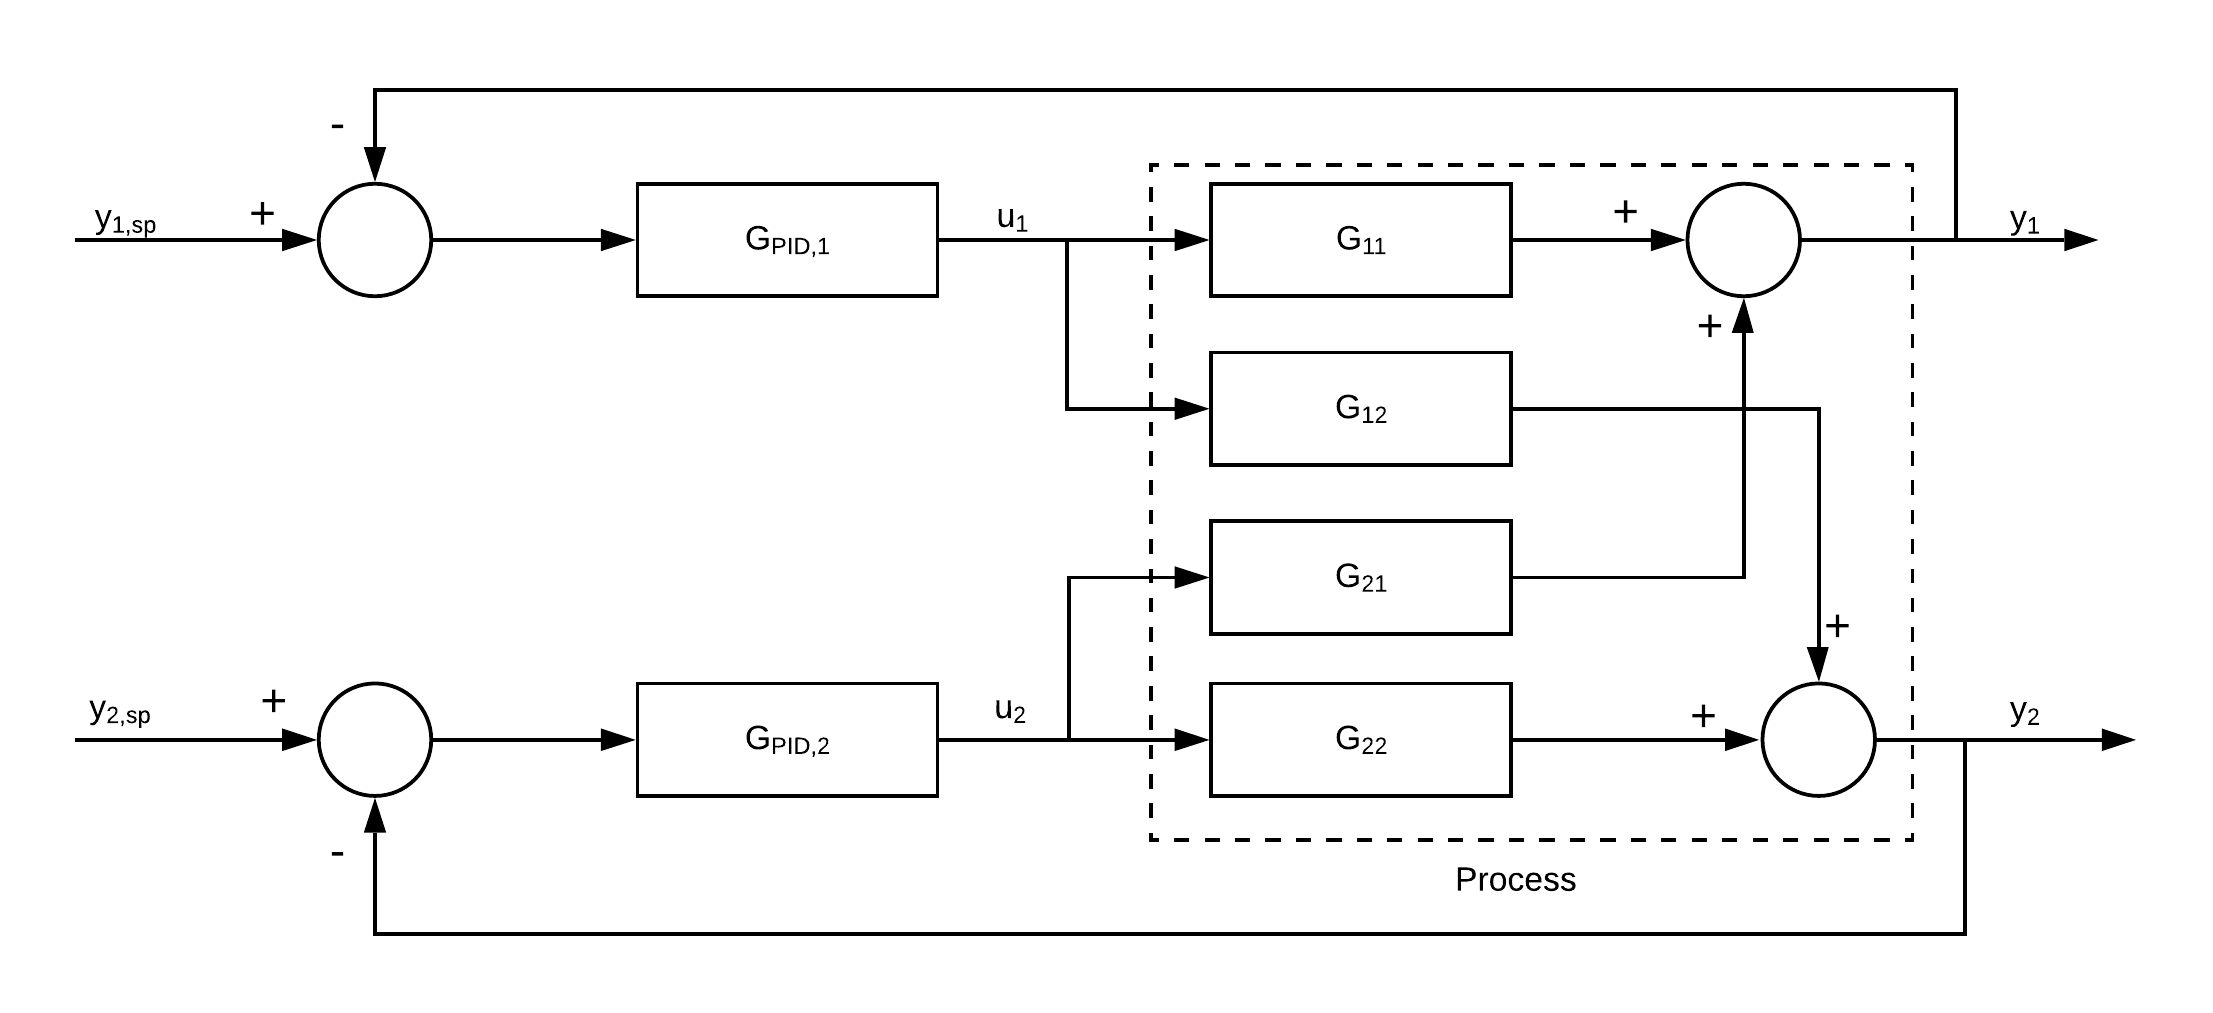
\includegraphics[width=\textwidth, keepaspectratio]{gfx/Chapter05/two_by_two_control_loop}
% %  \caption{A block diagram of a 2x2 control system. $G$ are process transfer functions representing the conversion of an input to an output in Laplace space.}
% %  \label{two_by_two_control_loop}
% %\end{figure*}

% \begin{table*}[bt]
%   \caption{Significance of RGA values. Reproduced from Shinskey \cite{Shinskey1984}.} 
%   \begin{tabular}{c l}
%     \centering
%     $\lambda_{ij}$ & Significance \\
%     \hline
    
%     <0 & Conditionally stable - do not close loop \\
%     0 & Control depends on other loop(s) \\
%     0-1 & Interaction extends period and raises gain \\
%     1.0 & No interaction with other loops \\
%     >1  & Interaction reduces control effectiveness \\
%     $\infty$ & Loops are completely dependent \\
%   \end{tabular}
%   \label{significance_of_rga}
% \end{table*}

% As shown in Table \ref{significance_of_rga}, Shinskey lists six different bands for the RGA, each with a different physical interpretation \cite{Shinskey1984}. A $\lambda_{11}$ value of 1.0 indicates there is no coupling between the two loops and is highly desirable.   Negative values mean that the system is only stable if the first loop is left open and the second is closed; this is because the second loop causes a response in the wrong direction. $\lambda_{11}$ values between zero and one can be tolerated, with preference for values closer to one. Large values represent significant coupling, with the extreme of infinity meaning the loops are completely dependent. This extreme case occurs when the two variables being controlled are necessarily dependent, such as steam temperature and pressure. It is important to note that interpretations for systems larger than 2x2 are not clear.

% The advantage of the RGA is that it only requires steady-state gains. These can be calculated from a simple open-loop pulse experiment or, if the plant is stable and close to steady-state, closed-loop plant data \cite{Pensar1993}. However, analyzing the steady-state behavior of a distillation column is usually not sufficient. Distillation columns are inherently dynamic, and a configuration that appears robust from steady-state analysis could be unstable in practice. Conversely, configurations that appear impossible at steady-state are often possible in the dynamic regime. 


% For example, Finco and Luyben completed a rigorous dynamic study on the optimal control configuration for a propylene/propane column and found that the unconventional D-B configuration worked most effectively \cite{Finco1989}. Steady-state simulations would suggest that the D-B configuration is not feasible because an overall mass balance on the column necessitates that only D or B can be fixed at a given feed rate (i.e., $F = D + B$) \cite{Skogestad2007}. This is evidenced by an infinite value of $\lambda_{11}$ for this configuration. However, in practice, Finco found that operators in an actual plant were implicitly using the D-B configuration and that, in general, high purity columns with components that have low relative volatilities (i.e., components with similar boiling points) are best controlled by the D-B configuration \cite{Finco1989}.

% These results suggest that dynamic analysis should be used in favor of steady-state analysis. McAvoy developed the dynamic relative gain array (DRGA), which uses a dynamic transfer function model to take into account the performance of the dynamic response \cite{Riggs2006}.\footnotemark The original DRGA sweeps across all frequencies of the transfer function model to find the dynamic response to different types of disturbances. A more recent method works with any dynamic model \cite{McAvoy2003}. It designs a simple optimal controller using the linear quadratic regulator and then uses partial derivatives of the closed-loop model to find the DRGA. When applied to an ill-conditioned 2x2 system and a nonlinear 4x4 system, the method was able to find the best pairings, whereas the RGA chose the incorrect pairings. 
% \footnotetext{The Cambridge University archives do not contain this paper, and the British Library Interloan Exchange has been shut down due to COVID-19. Therefore, descriptions in other papers and textbooks are relied upon for this summary.}


%\begin{itemize}
%	\item The method that Jan mentioned in my viva
%	\item The method from the Braatz group: https://aiche.onlinelibrary.wiley.com/doi/full/10.1002/aic.14107
%	\item The self-optimizing control methods from Skogestad
%	\item The multiobjective optimisation method from Yi Cao
%	\item The branch and bound method in the thesis
%\end{itemize}
%
%%In cases where an accurate dynamic model is available, the DRGA offers a promising method.  However, at the pilot plant stage, it is difficult to access accurate dynamic models.  Vapour liquid equilibrium data is often not available, and the behavior of a specific column might not be known (e.g., valve characteristics, heat-transfer coefficients, component aging, fouling, etc.). Despite half of a century of research, choosing control pairings is still a difficult and non-automatic procedure that cannot be carried out online. In contrast, PID tuning is a necessarily online procedure.
%
%Out of all the methods available, branch and bound is most promising due to its generality. What I"m not sure about is if we can use it here....could I reimplement that method myself and use it on flow chemistry distillation?

% In this work, one control configuration is assumed for a distillation column, but in future work, one of the above heuristics will be used to select a controller configuration prior to the following step of controller tuning.

\subsection{Tuning decentralized controllers}
Each of the decentralized PID controllers needs to be tuned. Tuning involves identifying the three parameters of the PID equation, $K^P$, $\tau_I$ and $\tau_D$:

\begin{equation}
    \label{eq:PID_defining_equation}
    u(t) = K^P e(t) + \frac{1}{\tau_I}\int_0^t e(t')dt' + \tau_D \frac{de(t)}{dt}
\end{equation}
where $u(t)$ is the controller output that is feed into the actuator (e.g., a valve) and $e(t)$ is the error at time $t$.
The parameters in Equation \ref{eq:PID_defining_equation} have intuitive explanations, which is one of the key advantages of PID control. $K^P$ is the proportional constant because it causes the actuator input to increase proportionally to the error. Proportional control gives fast responses to disturbances (e.g., an increase in flowrate upstream of a distillation column) but will always result in the controlled variable being offset from the setpoint. $\tau_I$ changes the amount of integral control, which helps remove steady-state offset.  Finally, $\tau_D$ varies the amount of derivative control, which helps prevent overshoot of the setpoint. Precisely, overshoot is the the maximum error after the value of the controlled variable has crossed the setpoint value. The goal of tuning is to maximize the speed of the dynamic response to disturbances while minimising the magnitude of overshoot and offset. 
    
As noted by several authors, though Equation \ref{eq:PID_defining_equation} is the textbook definition for a PID controller, the actual implementation of PID can vary significantly between different hardware manufacturers \cite{ODwyer2009, KiamHeongAng2005}.  O'Dwyer identifies nine different classes of PID algorithms used by industrial controllers \cite{ODwyer2009}. For example, some controllers include a low-pass filter on the derivative term to prevent drastic changes in error response. Algorithms used to tune PID controllers often assume a particular form of the PID equation, which is important to consider when choosing an algorithm for tuning a PID controller.  

Here, the literature on PID tuning is divided into three areas: heuristic tuning, Internal Model Control (IMC) tuning, and optimisation based tuning. This is not an exhaustive list, but instead a survey of the most commonly used techniques as well as those with potential to be fully automated.  

\subsubsection{Heuristic tuning}
A wide range of heuristic methods have been created based on the experience of operators or engineers in the field. The most well-known and widely used technique is the Ziegler-Nichols (Z-N) tuning method, developed in 1942 \cite{Ziegler1942}. It is known to deliver fast responses to disturbances and can be run directly on a process \cite{Riggs2006}. Z-N works by turning on P action only and increasing the proportional gain ($K^P$) until oscillations result. The minimum gain that causes oscillations is known as the ultimate gain $K_u$, and the period of the oscillations is known as the ultimate period $P_u$. These two parameters are then used in the relationships shown in Table \ref{table:ZN_parameters} to find the PID parameters.

\begin{table}[b]
	\centering
	\caption{Tuning parameters for the Z-N method. $K_u$ is the ultimate gain, and $P_u$ is the ultimate period.}
	\label{table:ZN_parameters}
	\begin{tabular}{ c c c c }
	& $K^P$ & $\tau_I$ & $\tau_D$ \\
	\hline
	P & 0.5$K_u$ & - & - \\
	PI & 0.45$K_u$ & 0.83$P_u$ & - \\
	PID & 0.6$K_u$ & 0.5$P_u$ & 0.125$P_u$ \\
	\end{tabular}
\end{table}

The advantages of Z-N and its refinements\cite{Hang1991} are that they do not require a process model. They can be easily implemented by an operator online, which perhaps explains their popularity \cite{KiamHeongAng2005}. However, it is often undesirable to introduce oscillations into a chemical process, which, if taken too far, could result in a loss of control (i.e., an unstable or runaway process). Relay feedback is an alternative method of obtaining $K_u$ and $P_u$, which only introduces small oscillations into the process \cite{Shen1994}. A relay is introduced into the control loop (i.e., an on-off switch).  The following process is executed: 
\begin{enumerate}
    \item A small step change is made in the input, u.
    \item The output y in monitored, and when it begins to rise, the input is changed to the negative of the step value.
    \item When the output crosses original steady state, the input is changed back to the positive value.
    \item 	This is continued, and the resulting oscillations are used to find the ultimate gain and period. Then, the Z-N parameters in Table \ref{table:ZN_parameters} can be used to find the PID parameters. 
\end{enumerate}

% \begin{figure}[bt]
%   \centering
%   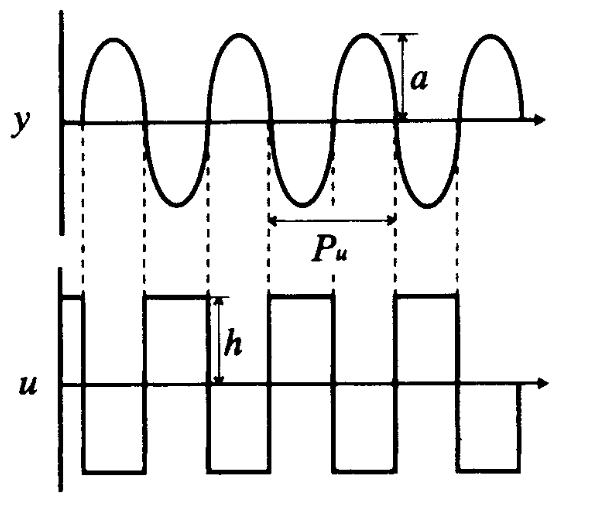
\includegraphics[scale=0.3]{gfx/Chapter05/relay_tuning.png}
%   \caption{Illustration of the relay tuning procedure for input $u$ and output $y$. Adapted from Shen et al \cite{Shen1994}.}
%   \label{relay_tuning}
% \end{figure}

Z-N and relay feedback methods are designed for SISO controllers in an independent environment. For decentralized MIMO control, previous work has shown that the Z-N rules in Table 1 give extremely aggressive tuning that causes oscillations when multiple controllers are introduced \cite{Riggs2006}. To compensate for this issue, Luyben introduced the BLT tuning method, which calculates a detuning factor $F$ to reduce the proportional gain of each controller \cite{Luyben1986}. $F$ depends on the number of loops being tuned, and Luyben's empirical simulations suggested that more nonlinearities in a system required higher values of $F$ (i.e., more detuning).

While heuristic methods are simple, they unfortunately often only work well for one type of process. Z-N, for example, works well for processes that can be explained by certain integral plus deadtime models \cite{ODwyer2009}. However, for  processes with strong nonlinearities, Z-N fails \cite{Hang1991}. This means that a different heuristic is needed for each type of process, and furthermore, the process type needs to be correctly identified. As a result there has been an explosion of tuning rules over the last thirty years, so large handbooks are needed to reference the rules \cite{ODwyer2009}. To compensate for the weaknesses of heuristic tuning, researchers have turned to other approaches.
 
\subsubsection{Internal model control tuning}
Internal Model Control (IMC) is a fundamental approach to controller tuning \cite{Skogestad2003}. Researchers have derived analytical equations for the controller parameters ($K^P$, $\tau_I$, and $\tau_D$) in terms of standard dynamic models. To tune a controller, process data is  fitted to the parameters of a dynamic model and, then, the appropriate analytical equation is used to calculate the controller parameters.

First-order plus deadtime (FOPDT) models are used as the starting point for IMC. These models represent the relationship between the input and output of a dynamic process as a first-order ordinary differential equation with deadtime ($\theta$). $\theta$ represents the time it takes for a change in input to begin affecting the output of the process. The standard FOPDT form is:
\begin{equation}
    \tau_P \frac{dy}{dt} + y = K_p u(t-\theta)
\end{equation}
where $\tau_P$ is the process time constant and $K_p$ is the process gain. $\tau_P$ represents the time for the output of a process to reach 63.3\% of its new steady state value after a step change in input, and $K_p$ represents how much a change in input will affect the output.  

Control models are often represented in the Laplace domain as transfer functions. The transfer function of the FOPDT model is:
\begin{equation}
    G_P(s) = \frac{K_p e^{-\theta s}}{\tau_p s +1}
\end{equation}
In many processes, the process time constant is significantly greater than the deadtime (called a lag-dominant process), so the FOPDT model can be simplified as follows \cite{Copeland2010}:
\begin{equation}
    G_P(s) = \frac{Y(s)}{U(s)} = \frac{K_p e^{-\theta s}}{\tau_p s +1} \approx \frac{K_p e^{-\theta s}}{\tau_p s } = \frac{K e^{-\theta s}}{s}
\end{equation}

As noted by Copeland et al. \cite{Copeland2010}., most IMC algorithms in the literature can be derived by combining the simplified FOPDT model above with the transfer function for a PID controller to get a standard form of the overall transfer function:
\begin{equation}
    G_O \equiv \frac{Y(s)}{u(s)} = \frac{[(2\lambda + \theta)s+1]e^{-\theta s}}{(\lambda s+1)^2}
\end{equation}
$\lambda$ is a tuning factor that determines the speed of the loop. A smaller $\lambda$ means a more aggressive control loop with faster responses. IMC tuning is often referred to as $\lambda$ tuning due to this factor. 

The difference between various IMC algorithms is how $\lambda$ is calculated. Each algorithm gives equations for the PID parameters with a tuning parameter, and the relationship between that tuning parameter and $\lambda$ varies. For example, in Skogstad IMC tuning, equations for the PI parameters can be written as follows\cite{Copeland2010}: 
\begin{equation}
    K^P = \frac{1}{K(\gamma +\theta)}
\end{equation}
\begin{equation}
    \tau_I = 4(\gamma+\theta)
\end{equation}
where $\lambda=2\gamma$. This is just one illustration that the tuning parameters in most IMC algorithms are scalar multiples of $\gamma$.

More recent work by Nandong et al. has extended IMC tuning to multiple control loops \cite{Nandong2013, Nandong2015}. The procedure relies on decomposing the process into modes using partial fractions and, then, designing a series of PIDF controllers (PID controllers with filters) for these modes. The method uses four overall parameters to tune any $n$ by $n$ MIMO system. To determine these four parameters, a heuristic based on frequency domain analysis can be used. Furthermore, an optimisation algorithm can be used to tune the four parameters until the integral error is minimised for all control loops. This method has been shown to give better results than BLT tuning for several  multivariable systems.  

IMC tuning is promising because it relies on a model of the process and analytically derived equations that guarantee stability. Furthermore, as shown by Copeland et al., a single equation can represent a whole class of processes accurately \cite{Copeland2010}. However, many assumptions are made when deriving the models, which is particularly problematic for nonlinear operations like distillation. Additionally, the multivariable technique developed by Nandong \cite{Nandong2015} still requires iteration and bears more resemblance to optimisation based tuning.

\subsubsection{Optimisation tuning}
The PID controller tuning problem can be posed as an optimisation problem.  The objective is a function of the error from the setpoint \cite{Pajares2019, Sumana2010, Rajapandiyan2012, Behroozsarand2012}, and the decision variables  are the PID parameters.  Hence, an optimisation algorithm can be used to iteratively approach an optimal set of parameters. Optimisation is, in some sense, a heuristic. The user must choose a form of the objective(s), which inherently determines how the algorithm manages the trade-off between fast responses, minimum overshoot and minimal offset. However, instead of a user deciding how to calculate a detuning factor or accurately model the plant dynamics, an algorithm guides to the same result using gradient descent or a heuristic (e.g., genetic algorithms). In the MIMO case, where there are strong nonlinearities, this automatic learning could be potentially useful. 

Various stochastic optimisation algorithms have been used previously because they do not require calculation of derivatives \cite{Sumana2010, Ganesh2010, Behroozsarand2012}, and some have global optimisation properties (i.e., they converge to the global optimum over time). Multiobjective genetic algorithms enable consideration of the tradeoffs between multiple optimal tuning strategies \cite{Behroozsarand2012, Pajares2019}. These optimal tuning policies are often called Pareto optimal points. In addition to GAs, gradient optimisation can be used \cite{Sommer2011}. It is not clear which methods work most effectively in general from the case studies.

One of the most important choices for optimisation is selection of the objective. For example, Sumana et al. use optimisation for tuning a multivariable PID control scheme for a reactive distillation column, and they sum the errors over  test cases with different disturbances \cite{Sumana2010}. By including multiple scenarios, the algorithm provides moderate performance on all cases, whereas the compared heuristics only work well for certain test cases. A variety of measures can be used including the integral squared error, integral absolute error, and integral time-weighted error. 

The potential disadvantage of optimisation based tuning is its inefficiency. Genetic algorithms often require hundreds of iterations to converge. This problem is not addressed in the literature because most papers are simulation based and simply do not need to be concerned with resource consumption. Overall, current methods for decentralized PID tuning rely on heuristics without guarantees, restrictive models or potentially inefficient optimisation methods.  This spurs us to evaluate an alternative procedure.

\section{Methods}
\begin{figure}
  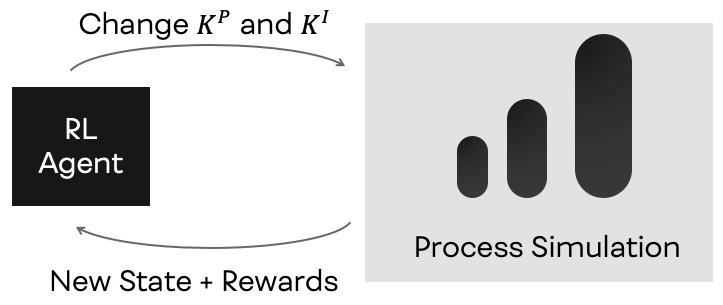
\includegraphics[width=\linewidth]{gfx/Chapter05/rl_tuning_loop.png}
  \caption{Schematic of the reinforcement learning and transfer learning process. An RL agent chooses the gain parameters for the PID controllers and receives rewards based on the behavior of the process.}
  \label{immalabel}
\end{figure}

Herein, RL is used to tune PID controllers for continuous chemical processes. The original hope was to train a RL agent in simulation and transfer to a real distillation column. As shown in Figure \ref{immalabel}, process simulations represent the environment, and the agent makes changes to the PID tuning parameters for this environment. 

\subsection{Representing a continuous process to an RL agent}
A chemical process can be viewed as an environment with multiple parameters that determine its performance. The parameters might be the sizing of the equipment, operating conditions, or the tuning of the control system; the performance might be measured in terms of throughput, stability or cost. In RL, changes to the parameters of the environment are called actions $\mathcal A$ because they are taken by an agent interacting with the environment. To know which actions to take, a RL agent needs a representation of the state $\mathcal S$ of the environment and rewards $\mathcal R$ for the actions it takes. The state of a continuous process can be represented by process data such as the error and oscillations in each control loop \cite{Lee2005, Badgwell2019, Shin2019}, while the reward is the performance. Whenever an action is taken, the new state is determined by the transition probability $\mathcal P$. Note that state refers to anything an RL agent observes about the environment, not just the thermodynamic state of a chemical process.

$\mathcal S$, $\mathcal A$, $\mathcal P$, and $\mathcal R$ are all components of a Markov Decision Process (MDP). In the MDP framework, the current state $s$ contains all the information an optimal agent needs to take an optimal action $a$.  RL can be phrased in several ways, but the approach taken here is to find a policy $\pi_{\theta}(s,a)$ that determines the distribution over actions given a state $s$:

\begin{equation}
	\pi_{\theta}(s,a) = \mathbb P[a|s,\theta]
\end{equation}
The policy is parameterized by $\theta$, which usually represents the weights and biases of a neural network. $\theta$ is learned through policy gradient algorithms, which define the gradient of the network loss $J(\theta)$ as:
\begin{equation}
	\label{policy_gradient_theorem}
	\nabla_{\theta}J(\theta) = \mathbb E_{\pi_{\theta}} [\nabla_{\theta} \log \pi_\theta(s,a)Q^{\pi_{\theta}}(s,a)]
\end{equation}
where $Q^{\pi_{\theta}}(s,a)$ is the value function that is trained to predict the expected future rewards, or return, of taking action $a$ from state $s$. Having the gradient of the cost in Equation \ref{policy_gradient_theorem} enables stochastic gradient descent to be used minimise the gradient, and thus find $\theta$ that give an optimal policy for the given MDP.

The MDP in this chapter is a simulation of a continuous  distillation column. The simulation is based on "Column A" by Skogestad and Morari in which a generic mixture with constant relative volatility of 1.5 is separated using a 41 stage column (including a reboiler and a condenser) \cite{Skogestad1988}. As shown in Figure \ref{lv_config}, the LV control configuration is applied, which means that reflux (L) or boilup (V) are available for composition control of the distillate or bottoms flows. Instead of measuring composition directly, temperature is often used as a proxy, which is the approach followed here \cite{Wolff1996, Luyben2006}. This is due to the strong link between temperature in the column and compositions of the outlet streams (i.e. distillate and bottoms) \cite{Luyben2006}. The temperature of stage thirty is controlled by the reflux rate. In the LV configuration, the distillate and bottoms flowrates are used to control the levels in the reboiler and condenser, which ensures the column is never empty and there is always continuous flow.  The level controllers are P-only, while the composition controller is in PI mode; derivative control is not used because it is most often useful for processes with very short time constants. The aim is to use an RL algorithm to take actions that change these four parameters such that the performance of the distillation column, or reward, is maximized.

Tuning occurs in episodes, where the RL agent updates the controller parameters every $n$ minutes and receives rewards for the tuning used in the previous $n$ minutes. Time resets to zero at the beginning of each episode. The update frequency was chosen to be every ten minutes based on the observation that changes to the controller parameters began to take effect within this time. As shown in Equation \ref{reward_function_1}, the reward function $R_t$ is a combination of the average normalized error $e_i(t)$ in $i=1 \dots N_c$ controllers and the number of oscillations in each the manipulated variables $p_i$. To calculate $p_i$, noise is removed using the Savitzky-Golay filter with a window length of 51 and polynomial order of three. This filter is used because it is commonly applied for filtering out high frequency noise from sensors; the parameters were selected via trial and error. The mean of the filtered signal is then subtracted to center the signal around zero, and the absolute value is taken. Finally, the number of local maxima with values greater than 1\% of the maximum variation in flowrate are summed. This method captures both damped and unstable oscillations.
\begin{gather}
	\label{reward_function_1}	
 	R_t = - \frac{1}{N_c t}\sum_{i=0}^{N_c}\sum_{\tau=0}^t \lvert e_i(\tau) \rvert  - \sum_{i=0}^{N_c}p_i\\[2em]
 	\label{reward_function_2}	
	\text{where}\;\;\; 	e_i(t) = \frac{\hat y(t) - \hat y_{setpoint}(t)}{\Delta \hat y_{max}}
\end{gather}

The state of the process simulation environment is represented as a $12\times 1$ array with the first four components as the proportional ($K_i^p$) gain constants of the three controllers and integral gain constant ($K_i^I$) of the temperature controller from the previous update. The next three components are the average normalized error from the setpoint $\bar E_i(t_1,t_2)$ in each controller $i$:
\begin{equation}
	\bar E_i(t_1, t_2) =\frac{1}{t_2-t_1}\sum_{\tau=t_1}^{t_2} \lvert e_i(\tau) \rvert
\end{equation}
The final five components of the state array represent the number of oscillations in the manipulated variables, feed composition, and feed rate. 

\subsection{RL agent}
Previously, the algorithms for training RL agents were only robust when simple linear functions were used to predict the relationship between states and actions, and empirically, working in continuous action spaces was not successful \cite{Sutton2018}. However, over the last ten years, several methods for training nonlinear functions were developed, enabling much more complex behaviors to be learned \cite{Mnih2013, Lillicrap2016}. These methods belong to a family of algorithms called policy gradient algorithms, which use neural networks as a policy that predicts a continuous action given a state. Training these networks relies on taking random samples of the experience of an RL agent to remove the time correlation and meet the independent and identical input distribution requirements for training nonlinear functions such as neural networks. If the MDP criteria are met and the state fully describes the history, then randomization during training will be effective. The proximal policy optimisation (PPO) was used \cite{Schulman2017} because it has strong performance across a wide range of tasks. PPO uses a KL divergenece penality to limit the amount the policy can be updated in any iteration, which prevents the policy from deviating into an undesirable action space in a single update and therefore failing to collect useful training data in subsequent steps \cite{Schulman2017, Engstrom2020}. To train the agent, random, but bounded oscillatory feed compositions and feed rate disturbances are simulated in each episode. This disturbance represents slow oscillating changes in feed rate $F$ and feed composition $z_F$ that often occur in continuous processes. For a given episode, the disturbance is as follows:
\begin{equation}
	F(t) = 
	\begin{cases}
		\underline F \;\; \text{if}\;\; t < 1200 \;\text{seconds} \\
		\underline F(1+ 0.2\cos(0.001t-1200))+\frac{1}{60000} \mathcal{N}(0,1) \;\; \text{otherwise}
	\end{cases}
\end{equation}

\begin{equation}
	z_F(t) = 
	\begin{cases}
		\underline z_F \;\; \text{if}\;\; t < 1200 \;\text{seconds} \\
		\underline z_F(1+ 0.2\cos(0.001t-1200))+0.001 \mathcal{N}(0,1) \;\; \text{otherwise}
	\end{cases}
\end{equation}
where $\underline F$ is the nominal feed rate and $\underline z_F$ is the nominal feed composition.

\subsection{Software implementation}
Discrete time PI controllers are implemented using the following form:
	\begin{equation}
	u_i(t+1) = K_i^P e_i(t) +K_i^I \sum_{\tau=0}^{t}{e_i(\tau)}\ 
	\end{equation}
where $u_i(t)$ is the output of controller, $K_i^P$ is the proportional gain, and $K_i^I$ is the integral gain. The controller output is used to scale the nominal flowrate by the maximum change in flowrate $\Delta L_{max}$:
\begin{equation}
	L(t) \leftarrow \underline L + u_i(t)\Delta L_{max}
\end{equation}

The output of the controllers is bounded in the range $[-1,1]$ to reflect that, in an actual process, the flowrate can only change in a finite range outside of its nominal range due to valve and pump limits. In practice, the integral term is also constrained because it can become very large when an actuator saturates, causing large changes in controller output upon desaturation of the actuator. This phenomena is called windup, and the constraint procedure is called anti-windup \cite{Riggs2006}, but we do not include any anti-windup protection here for simplicity.

Normalization of states and actions can improve the performance of an RL algorithm \cite{Engstrom2020}. This is due to the assumption that the inputs outputs of the policy network will be identically and independently distributed (i.i.d.).  The i.i.d. requirement is met by scaling the state and action arrays in the range $[-1,1]$ based on bounds that are set \emph{a priori}. The bounds on the controller parameters in the state and action arrays are set by taking a confidence interval around an estimate of the process gain $K_i^{Process}$ or time constant $\tau_i^{Process}$ for a particular input-output pairing\cite{Cai2009, Astrom2006}:

\begin{equation}
	[K_i^{P, low}, K_i^{P, high}] = \Biggl [\frac{1}{ K_i^{Process}}-10 \frac{1}{\vert K_i^{Process} \vert}, \frac{1}{K_i^{Process}}+10 \frac{1}{\vert K_i^{Process} \vert}\Biggr ]
\end{equation}
\begin{equation}
	[K_i^{I, low}, K_i^{I, high}] = \Biggl [0, \frac{10}{ \tau_i^{Process}}\Biggr ]
\end{equation}

Empirically, this was a sufficiently wide range for the algorithm to be able to to explore negative and positive gain constants as well as smaller and longer reset times. The errors $e_i(t)$ were already scaled in  $[-1, 1]$ (see Equation \ref{reward_function_2}). The number of local minima and maxima (i.e., oscillations) was normalized by ten times the number of integration steps in a RL step, which proved to be a sufficiently large range. 
 
The aformentioned Column A model, PID controllers and RL algorithms are implemented in python. The RK45 integration method in SciPy is used for solving the distillation column model \cite{2020SciPy-NMeth}, and the python package simple-pid is utilized for modeling PID controllers \cite{Lundberg2019}.The implementation of PPO is taken from the OpenAI spinning up package. The environment implements a step method that takes actions from the RL algorithms (i.e., new controller parameters) and outputs the new state and rewards after stepping forward ten minutes in simulation time. The RL algorithms iteratively call step until the environment determines an episode is terminated. Episodes are terminated at the maximum episode time. Training of a policy with two layers of twelve hidden units required approximately three hours on a machine with 16 parallel workers. The learning rate of the value and policy networks was 1e-4. Other simulation parameters are shown in Table \ref{parameters_table}.

\begin{table}[bt]
  \caption{Values of parameters used for distillation column simulations. Code Name refers to the name of the variable in the software.}
  \begin{tabular}{cccc}
    Variable & Code Name & Units & Default \\
    \hline
    $\Delta t$ & step\_time & seconds & 600  \\
    $N_T$ & n\_stages &  & 41 \\
    $k$ & feed\_stage & & 20  \\
    $\alpha$ & alpha & & 1.5  \\
    $\underline F$ & nominal\_feed\_rate & kmol/second & 0.0167  \\
    $\underline z_F$ & nominal\_feed\_composition & & 0.5   \\
    $\underline q$ & nominal\_q & & 1.0 \\
	$\underline{R_R}$ & reflux\_ratio & & 5.41 \\
	$\underline D$ & nominal\_distillate\_rate & kmol/second  & $0.5 \underline F$ \\
    $\Delta L_{max}$ & flow\_delta & kmol/second  & 0.005  \\
	$\tau_l$ & tau\_l  & seconds & 3.78  \\
	$\lambda$ & lambd\_a & & 0 \\
	$K^{Process}_{reboiler}$ & kp\_reboil\_level & seconds & -0.333  \\
	$K^{Process}_{condenser}$ & kp\_codenser\_level & seconds &  -0.333\\
	$K^{Process}_{temperature}$ & Kp\_temperature & seconds deg C/kmol & -0.021 \\
	$\tau^{Process}_{temperature}$ & Taup\_temperature & seconds & 7200 \\
  \end{tabular}

  \label{parameters_table}
\end{table}


\section{Results and discussion}

\begin{figure*}[tb]
  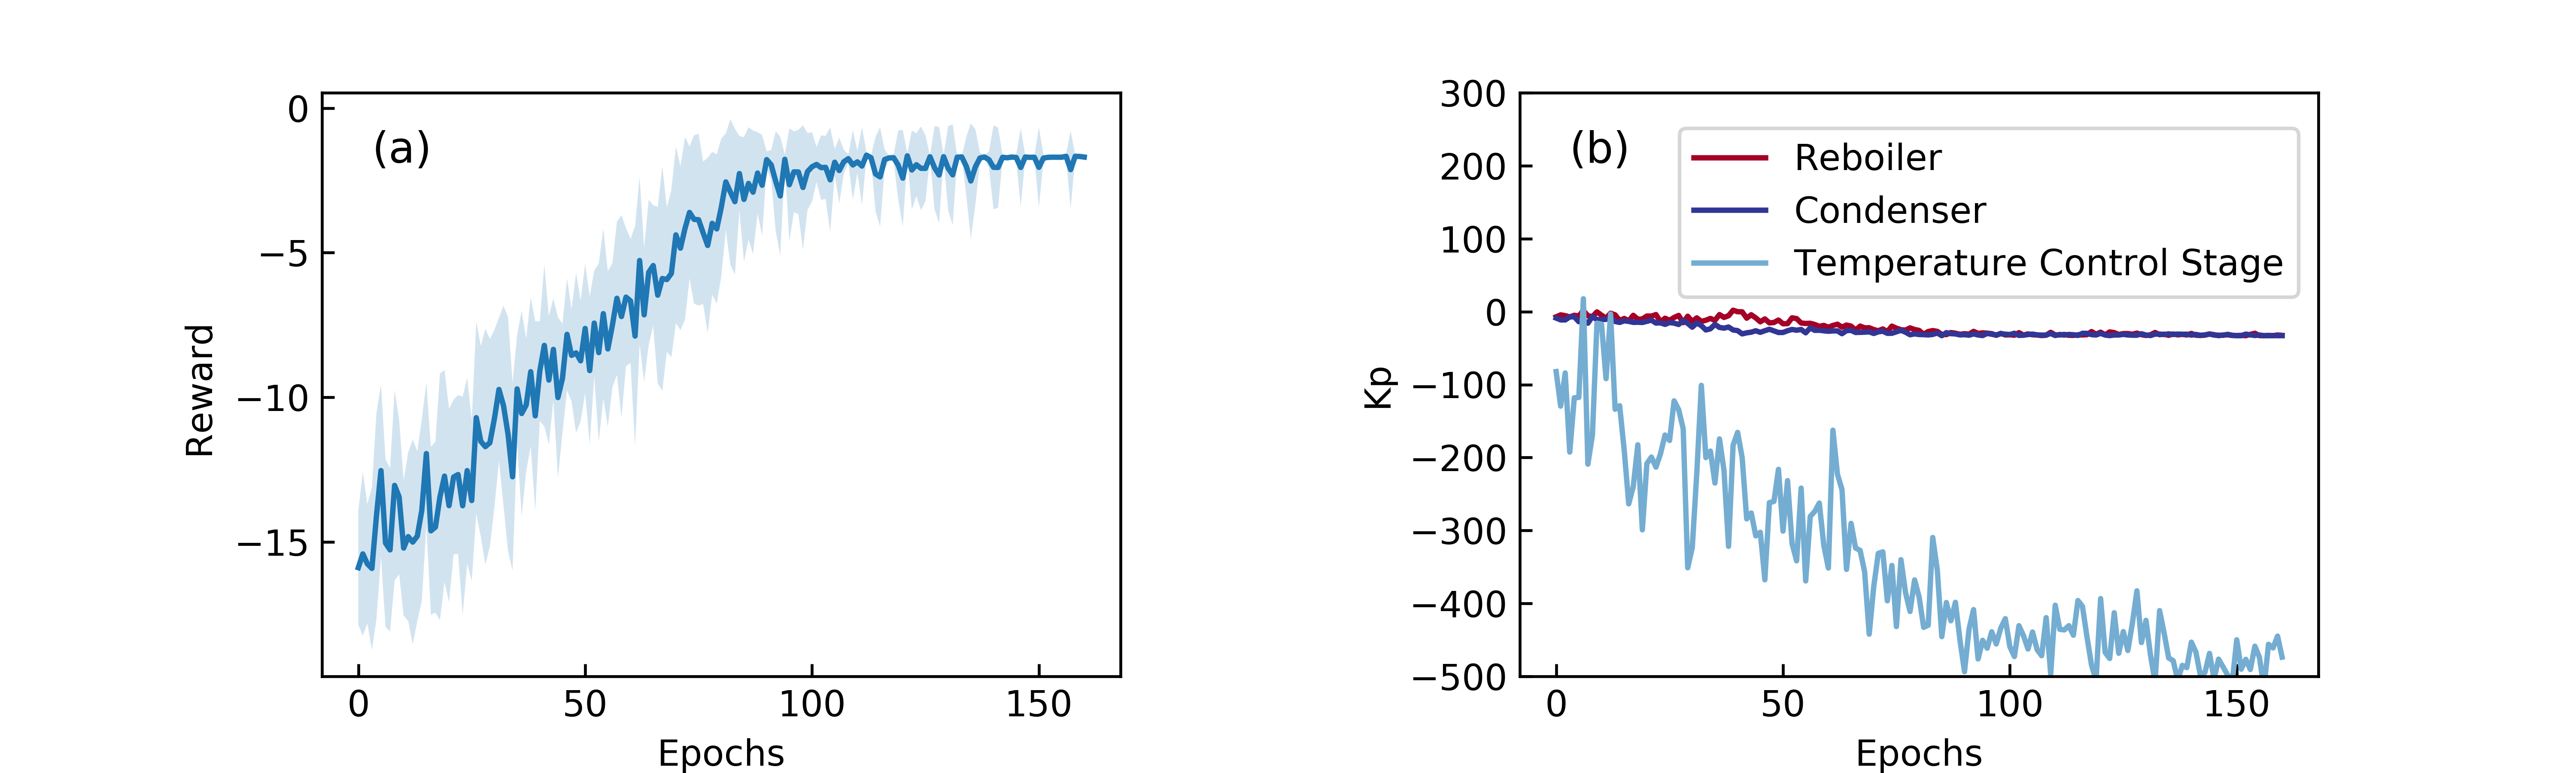
\includegraphics[width=\textwidth]{gfx/Chapter05/dis3_74_reward_parameters.png}
  \caption{An RL agent was trained to find the optimal tuning parameters for a distillation column using the proximal policy optimisation (PPO) algorithm over approximately 77,000 steps. (a) Average reward improves over the course of training. As the training continues, the agent learns to select parameters that favor distillation column stability and minimal controller error. (b) The controller gain parameters stabilize over the course of training.}
  \label{ppo_training_curve}
\end{figure*}

An RL agent was trained using the PPO algorithm to tune the parameters of controllers on a dynamic simulation of a distillation column. As shown in Figure \ref{ppo_training_curve}a, the agent learned by itself to tune the controllers for a distillation column. At first, it took random actions, but as the training progressed, the underlying policy became better able to predict how to change the controller parameters based on the state of the last step (i.e., ten minutes in the simulation). As shown in Figure \ref{ppo_training_curve}b, the controller parameters stabilized over the course of training. This indicated that the algorithm had finished exploring and was then able to exploit. Furthermore, the column parameters had the correct signs that would be expected for this control system.

\begin{figure*}[p]
  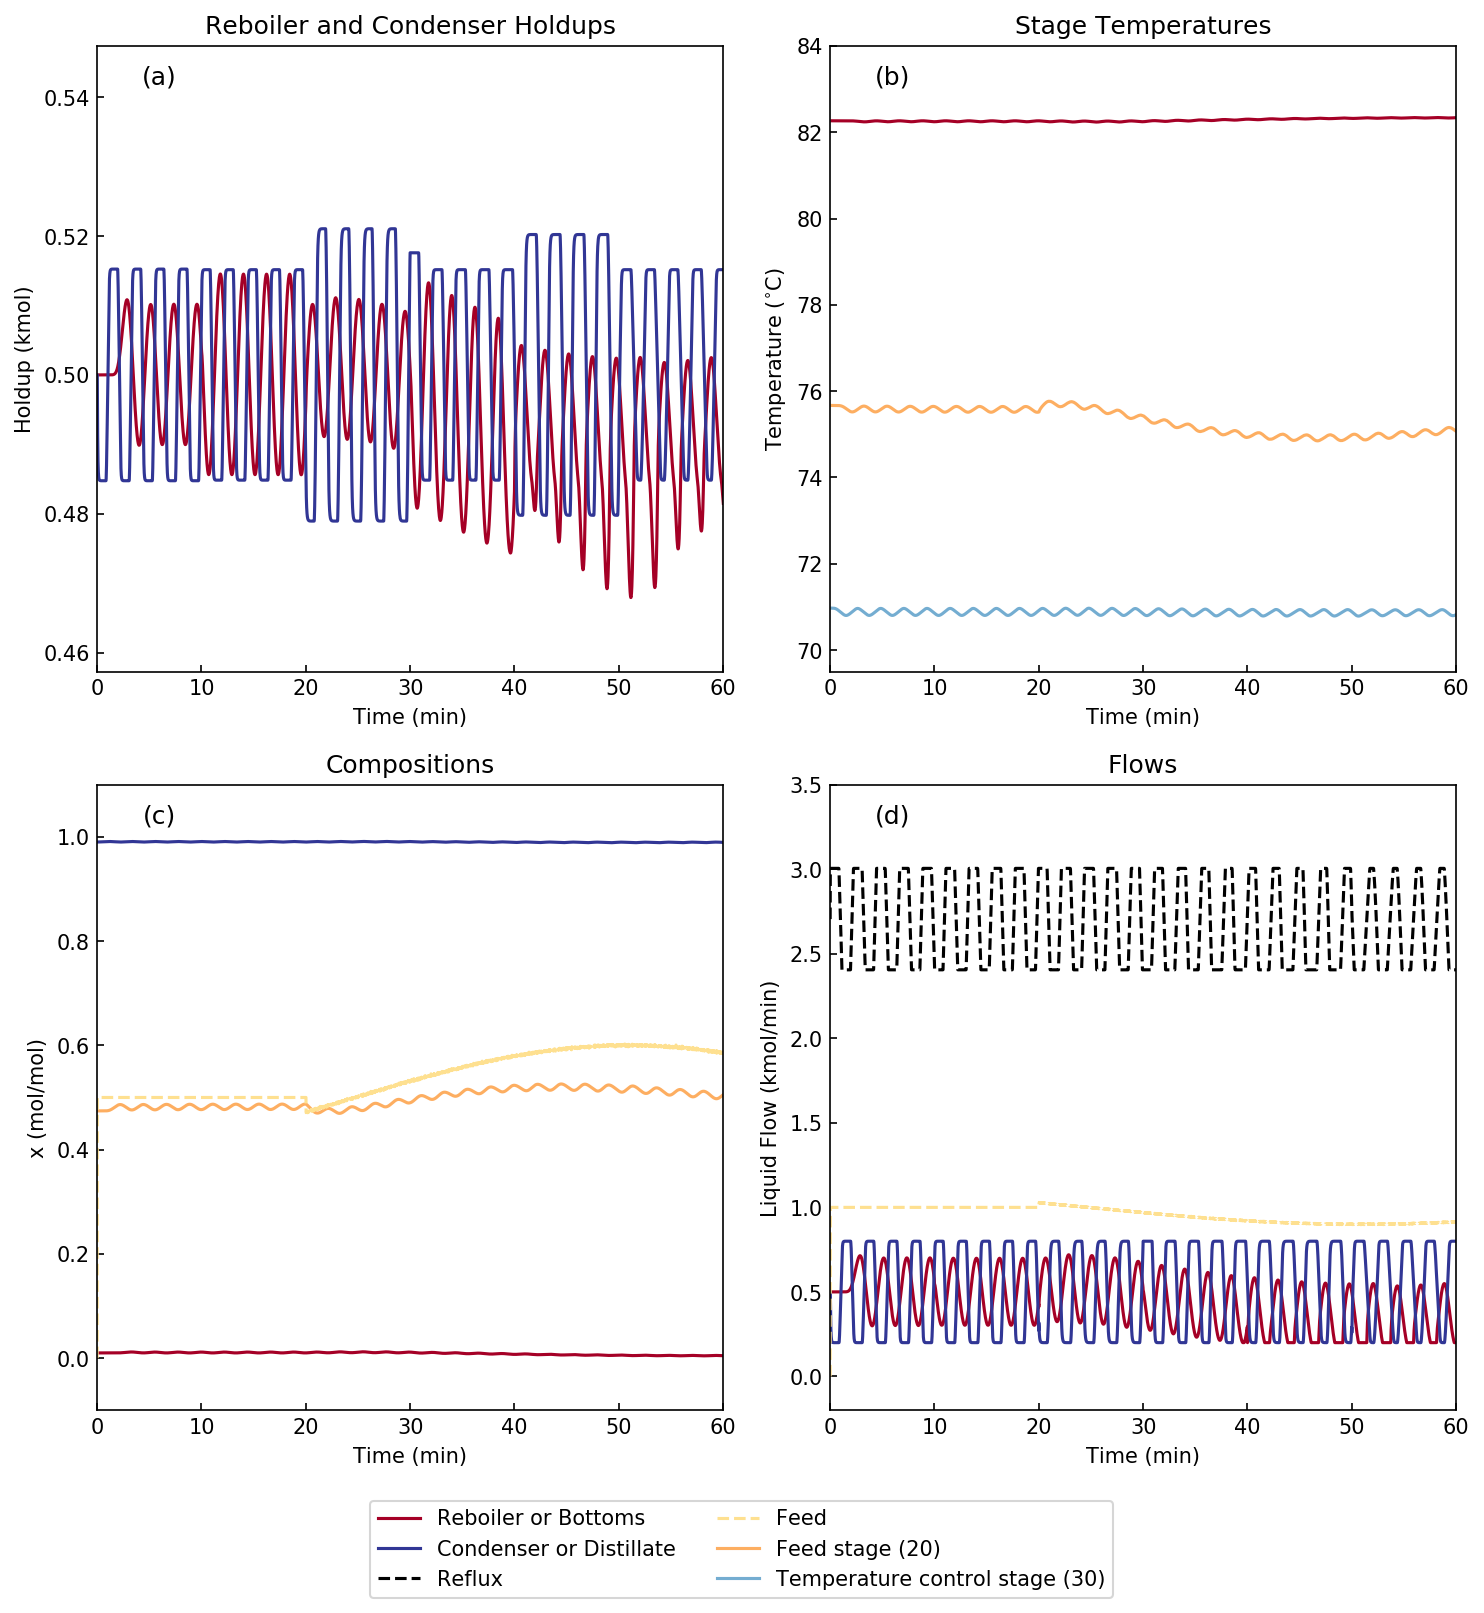
\includegraphics[width=\textwidth]{gfx/Chapter05/20200424_trained_policy_sixty_minutes.png}
  \caption{Results of controlling Skogestad Column A using the LV configuration with inferential composition control via temperature on stage 30 for sixty minutes of simulation time. An RL agent was used to select tuning parameters. (a) Holdup of the reboiler and condenser over time. The setpoint for both values is 0.5 kmol. (b) Stage temperatures over time. Stage 30 is controlled at $70^{\circ}$C, a value determined via steady state simulations. (c) The compositions in the feed, distillate and bottoms over time. (d) Liquid flows in the feed, reflux, distillate, and bottoms.}
  \label{trained_policy}
\end{figure*} 

However, as shown in Figure \ref{trained_policy}, when the trained agent was applied to the column after training, there were significant oscillations in the controlled variables. Figure \ref{trained_policy}a shows that the holdups oscillated more than 20 \%, and Figure \ref{trained_policy}b illustrated that the controlled temperature stage was varying significantly. This was caused by a high gain in the temperature control loop (Figure \ref{trained_policy}c and d). Consequently, there were nearly 20 \% oscillations in the reflux flow rate which resulted in oscillations in condenser holdup (as the reflux came from the condenser). Thus, the tuning of the temperature control loop had an influence on the level control loop and vice versa. Furthermore, thousands of tuning iterations were required to find optimal tuning parameters, which is not practical in a real distillation column.

\begin{figure}[t]
  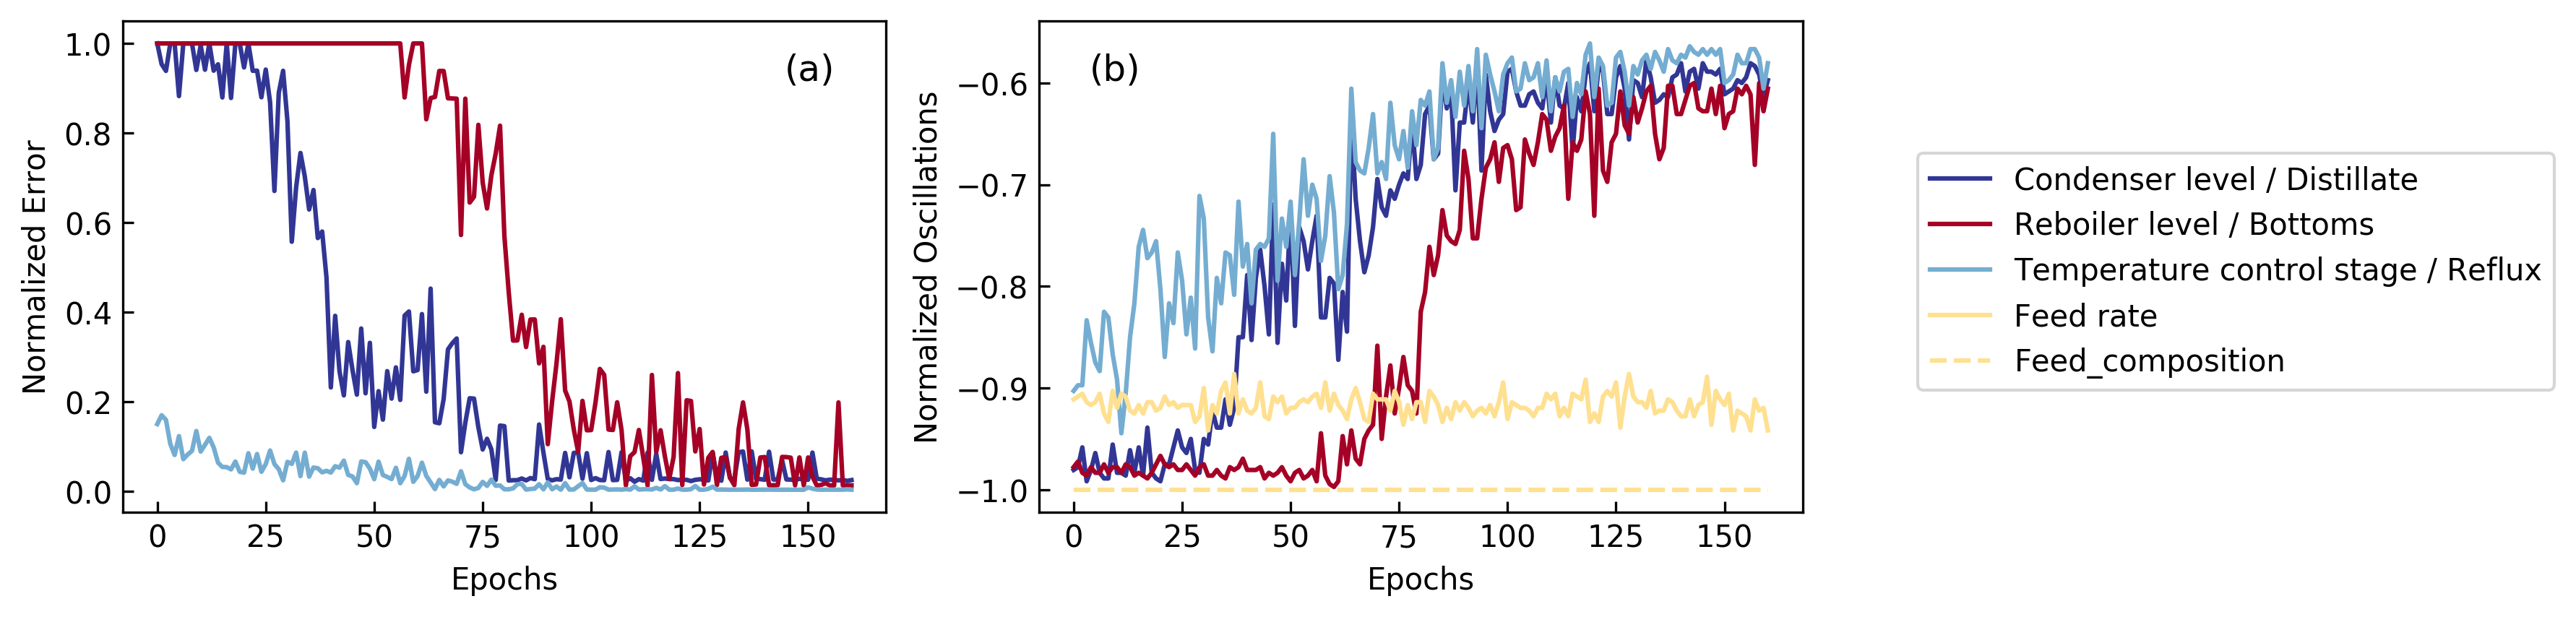
\includegraphics[width=1.2\textwidth]{gfx/Chapter05/dis3_74_errors_oscillations}
  \caption{Normalized error and oscillations in the control loops and feed.}
  \label{errors_oscillations}
\end{figure}

Figure \ref{errors_oscillations}a shows that the normalized error in all control loops decreased over training. However, as shown in Figure \ref{errors_oscillations}b, the normalized number of oscillations in the distillate, bottoms, and reflux flows increased on average, while the feed rate and composition had very few oscillations. The discrepancy between oscillations in the feed and other flows illustrated that the oscillations were being introduced by the control system and not the external disturbances. This was particularly problematic since the reward continued to increase despite the worsening oscillations. In other words, the agent was encouraged to introduce more oscillations into the system by increasing the magnitude of the gains.

The simplest remedy to this problem would be to incentivize the agent to reduce oscillations. As shown in Figure \ref{reward_tradeoff}a, the oscillations term in the reward was an order of magnitude smaller than the error term at the beginning of training. Only near the end of the training, when the policy had stabilized, did the error and oscillations reach the same magnitude. An experiment was conducted where the oscillations term in the reward function was multiplied by ten. As shown in Figure \ref{reward_tradeoff}b, the temperature control proportional gain selected by the agent trended positive over the training, which was the wrong sign for this parameter. This indicated that simply changing the weighting of the oscillations term would not solve the problem.

The use of P-only control on the level controllers was consistent with the academic literature\cite{Skogestad1988} but not practical in actual distillation control. Astrom noted that P-only control required specification of the correct bias in the controller output to achieve zero steady state error \cite{Astrom2006}. A more robust alternative would be to include the integral term, which acted like a continuously adjusting bias.

The time constant of Skogestad Column A is approximately 194 minutes \cite{Skogestad1988}, and, as shown in Figure \ref{trained_policy}c, the feed disturbances used in this simulation are slow and oscillatory. The ten minute updates are unlikely to capture these disturbances. When there is not sufficient information in a single update of the state to predict actions, the problem no longer meets Markov criteria and becomes a partially observed Markov decision process (POMDP). In other contexts, researchers have applied RL to POMDPs by replacing the feedforward neural network policy with a recurrent neural network (RNN) policy that takes account of previous state updates \cite{Bakker2002, Hausknecht2015}. In fact, recent work demonstrated that a particular type of RNN, long short term memory (LSTM) networks, have superior performance to feedforward networks on POMDPs \cite{openai2018}. Furthermore, it might be possible to learn the best descriptors of the process directly from time series data using a convolutional kernel and feed these descriptors to an LSTM \cite{Hausknecht2015, Badgwell2019}. This would ensure that data summary methods (e.g., averaging the error) do not result in insufficient state information. 

\begin{figure}[t]
  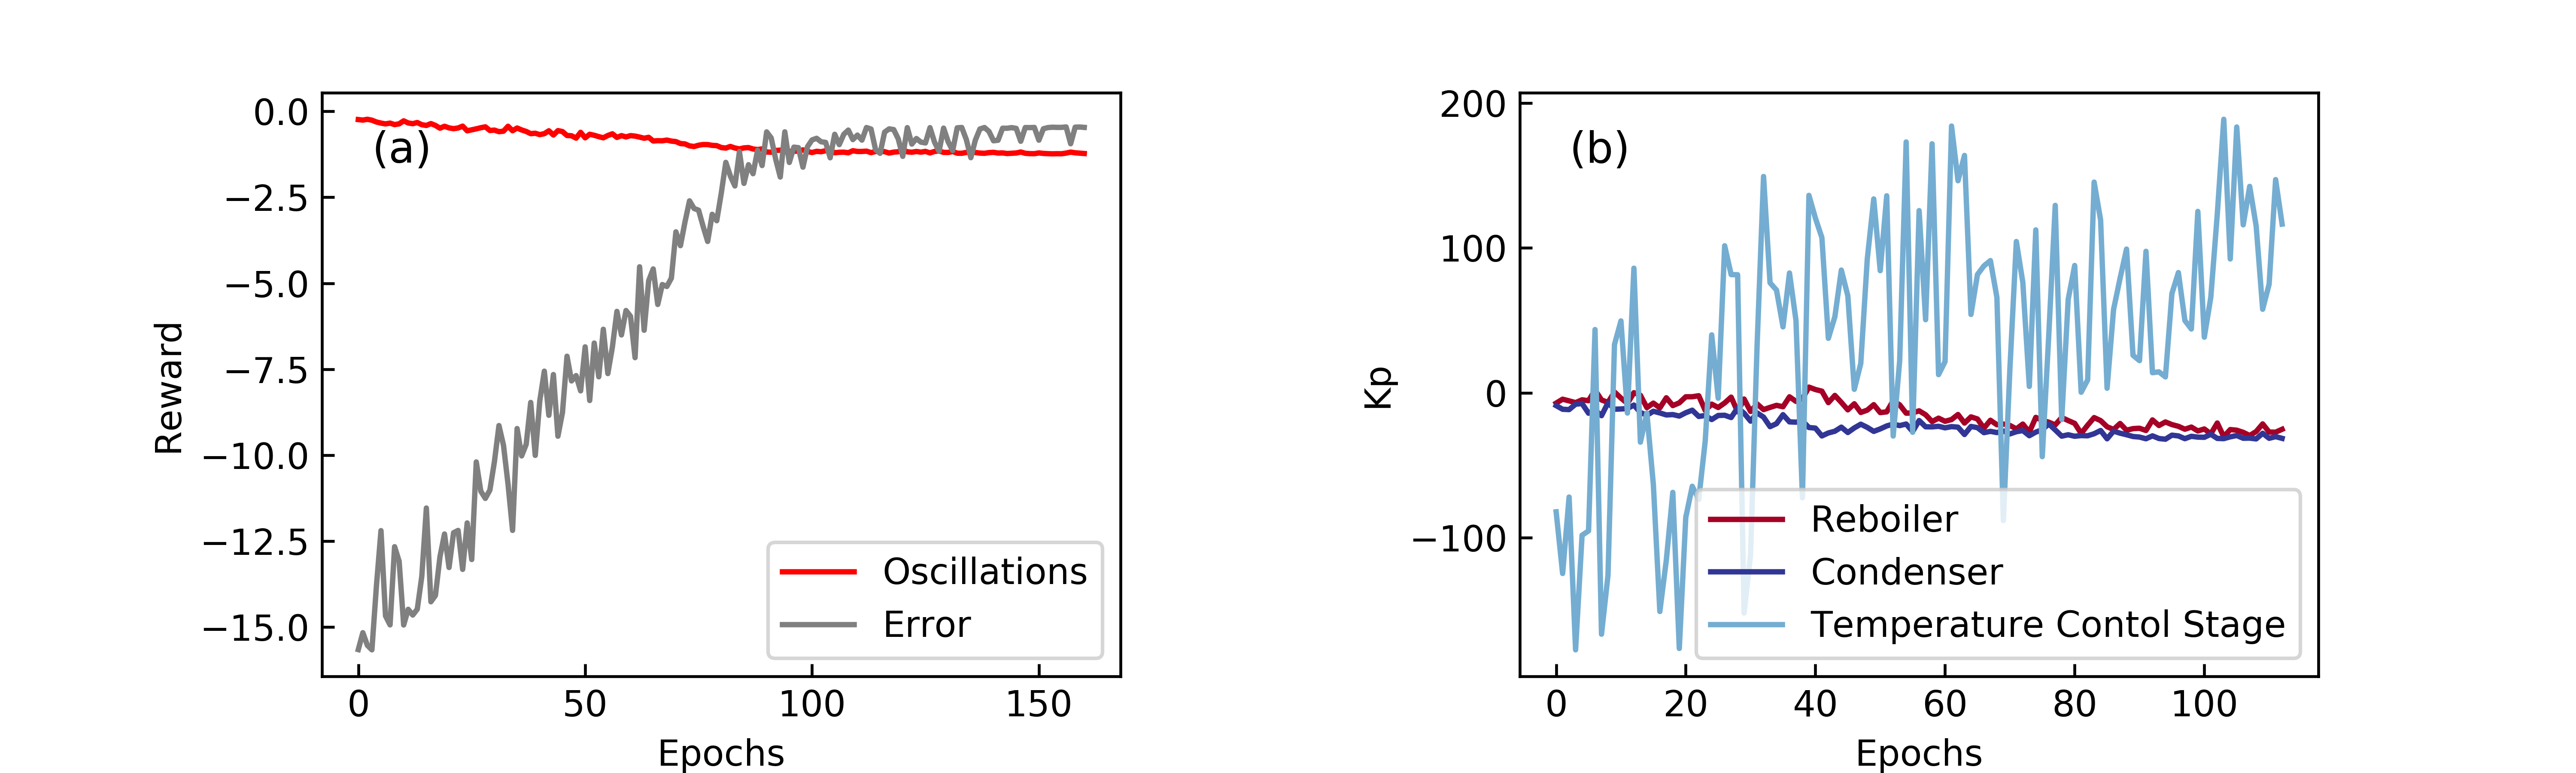
\includegraphics[width=1.2\textwidth]{gfx/Chapter05/oscillations_study.png}
  \caption{Study on removing the oscillatory behavior of the RL tuned control system. (a) The different components of the reward function over the course of training with standard weighting. (b) Results from an experiment with increased weighting of the oscillations term in the reward function.}
  \label{reward_tradeoff}
\end{figure}

% Changing the type of disturbance applied during training to better reflect those using in the laboratory could also enable better agent performance. Oscillatory disturbances are notoriously difficult to attenuate using PID controllers, so step disturbances are commonly used during tuning to give a monotone input-output relationship \cite{Astrom2006}. However, using step disturbances of varying magnitude would likely enable the agent to learn more effectively as there would be sufficient information to implicitly learn a model of the distillation column. 
 
A final challenge is due to the specifics of the dynamic models of continuous processes. The simple Column A model used here does not include energy balances or commonly observed phenomena such as flooding \cite{Nooraii1998}.  Therefore, the behavior learned by the agent might not transfer well to an actual distillation column. This is a severe limitaton that I address in the next chapter.

\section{Conclusions}

In this chapter, I introduced the challenge of controller tuning for distillation columns and introduce a set of experiments to that attempted to apply RL to controller tuning. I found that the RL agent was unable to find optimal tuning parameters despite thousands of iterations. While it might have been  possible to improve the performance of the RL tuning, several challenges with the approach led to the halting of the project:

\begin{itemize}
    \item RL requires many iterations to find optimal policy. Even the simulation training can take hours to days on fast computer.
    \item RL trained on a specific configuration is not transferable. A new agent would need to be trained for each new configuration of the distillation column, which is unacceptable given the above training constraint.
    \item Applying the trained policy to the laboratory might be impossible. At the time of writing, RL agents had not been deployed in chemical plants and, therefore, did have the same safety verification of other techniques such as model predictive control. 
\end{itemize}

 Overall, these conclusions led me to try a transfer learning approach based on rigorous dynamic simulation and Bayesian optimisation.
